\documentclass[10pt]{report}
\usepackage{fullpage,listings,amsmath}
\usepackage{pdflscape,setspace,graphicx,textcomp,picins}
\usepackage[colorlinks=true]{hyperref}


\lstnewenvironment{code}{\lstset{language=haskell,basicstyle=
\renewcommand{\baselinestretch}{1}\footnotesize}}{}


\title{Integrated Analysis of Room Performance}
\author{Michael Novak} %, Shaun Brandt, Mandar Patil, Hema Kumar, and Yu Yang}


\begin{document}

  \maketitle
%\doublespacing
\section{Automated Analysis}
The figures and tables in this document were created by \href{run:analysis.hs}{analysis.hs}; functions acting on the raw data produce \LaTeX{} \& {\tt gnuplot} files, which are rendered as tables and figures; 
the colors used in the plots were the carefully chosen colors\footnote{\url{http://www.sron.nl/~pault/colourschemes.pdf}} to be distinguishable. 


\begin{itemize}
  \item Postmortem data gotten from \verb=/u/karavan/Public= at \verb=rita.cat.pdx.edu=
  \item \date{2011-05-05}---The Low Density Workload---\verb=LD_A1_56p_2ppn_28n_IO-BASIC_even_RAWDATA=
  \item \date{2011-04-25}---The High Density Workload---\verb=HD_A1_224p_8ppn_28n_RAWDATA=
\end{itemize}

\section{Data}
We've been given postmortem data, \verb=LD_A1_56p_2ppn_28n_IO-BASIC_even_RAWDATA=, corresponding to the experiments described in \cite{Karavanic2011}:
\begin{itemize}
  \item
 \begin{quote}
Low Density Even Distribution -- In this set, we used
racks B1, B2, B3, and B4; and we scheduled two MPI
tasks per node, using all of the nodes in all four racks.
 \end{quote}
 \item
\begin{quote}
In the low density LD schedules, the 224 processes executed on 112 nodes, with two processes per node, and the processes were spread across racks B1, B2, B3, and B4.
 \end{quote}  
 \item
   \begin{quote}
     The nodes are connected via a DDR InfiniBand 1-layer fat tree; one rack (A2) contains the networking equipment and seven racks (A1, A3--4, B1--4) are for the compute nodes.
   \end{quote}
 \item
   \begin{quote}
     \emph{Power.} We collect power per rack, at 10 second intervals. This is converted by FRED to kWh.
   \end{quote}
 \item
   \begin{quote}
     \emph{Cooling.} Each spray-cooled rack has a Thermal Management Unit (TMU) which contains pumps, a liquid-to-liquid heat exchanger, and control electronics.
   \end{quote}
 \end{itemize}

 \section{Power \& Cooling}

 Figure 1 shows power consumption, in kWh (7.63\textcent{} per kWh, in Oregon), for the racks used in the trials. It was hard to tell whether the gradient of one line was steeper than another; hence the accompanying tables were created to show overall kWh increase per trial, and to further scrutinize power consumption within the racks. 

The tables, within Figure 1, can be used to compare how the two air-cooled racks ($A_1,A_2$) faired, energy performance-wise, against the water-cooled racks ($A_1,B_1,\dots,B_4$). Note: our data seems to be corrupted by faulty sensor readings; at some nodes, in certain racks, sensor readings gave negative temperature values; these readings were discarded; so the average temperature does not include every node in every rack; and, most temperature readings remained static with time, which made calculating the average trivial.

For the water-cooled racks, Figure 2 is a visualization of TMU utilization for each trial (t01--03)\footnote{Within {\tt RAWDATA}, the application and system level data for each trial are in the trial directories: t1, t2, t3.}: the degree of cooling which the TMU provided, captured by the water-temperature-delta metric; and the mass flow rate of water, captured by the manifold pressure metric. 
TMU utilization metrics were collected by FRED at 10 second intervals; so, for simplicity, each trial's time series starts at 0 and is incremented accordingly.

%Evidently, trial 3 (t03) involved slightly more energy intensive application processes.

%Are we ever going to get PerfTrack and have the data organized in PostgreSQL?
%perhaps it will be easy to gather the data necessary to make a chart like the one depicted on page 440 of \url{http://web.cecs.pdx.edu/~karavan/cs533/karavanic_PDCS2011.pdf}.


 \subsection{Chillers}
Within the cooling infrastructure, most of the energy is spent on chillers, which refrigerate the coolant---water, in our case---used to extract heat from the equipment in the data center.
 The following metrics, derived from \cite{Patnaik2009}, are displayed in Figures 3 \& 4. Chiller utilization measurements were collected by FRED at 30 second intervals; so, for simplicity, each trial's time series starts at 0 and is incremented accordingly. Note: only three chillers units ($C_1,C_2,C_4$) were turned on during the trials, as evidenced by KW consumption---$C_3$ and $C_5$ were turned off. 
 \begin{itemize}
   \item
   {\bf IT cooling load.} This is the amount of heat that is generated (and thus needs to be dissipated) at a data center. It is approximately equivalent to the power consumed by the equipment since almost all of it is dissipated as heat. It is commonly specified in kilowatts (KW).
 \item
   {\bf COP.} The coefficient of performance (COP) of a chiller unit indicates how efficiently the unit provides cooling, and, is defined as the ratio between the cooling provided and the power consumed, i.e.,
   \begin{equation}
     COP_i = \frac{L_i}{P_i}\label{cop}
 \end{equation}
where $L_i$ is the cooling load on the $i$th chiller unit and $P_i$ is the power consumed by it.
\item {\bf Chiller utilization.} Chiller utilization depends on the degree of cooling provided; i.e., the difference between the inlet and outlet water temperatures.
\end{itemize}



 \section{Data Mining}
 If only we had access to more data\dots
 \begin{itemize}
     % \item It would be nice if we could get at the FRED measurements through a cloud-based data store---perhaps a graph database.  
   \item It would be nice if FRED measurements were stored in a NoSQL graph database. A NoSQL database would be much faster than PostgreSQL. And having the data structured as a graph seems like it would make the data easier to navigate.
   \item We could compare high-density workload with low-density workload; and , perhaps medium-density workload---if it exists.
    \item We could try to use the temporal data-mining techniques in \cite{Patnaik2009,Patnaik2011} on TMU and Chiller data. But we might need longer time slices; no motifs can be seen at such a fine granularity---within just 3 sets of 9 minute trials---clustering would just produce nonsense.
   \item \cite[p. \;34:7]{Patnaik2011}
     \begin{quote}
Motifs are repetitive patterns of occurrence in time-series data. In understanding multivariate time-series data about chiller utilizations, we seek to identify motifs that underly how different chillers are involved in meeting the varying demand posed by data centers. We would like to identify regions of time-series progression that demonstrate better/improved sustainability measures than others.
     \end{quote}
   \item \cite[pp.\;1308--1309]{Patnaik2009}
 \begin{quote} 
   A multivariate time series $T = \langle t_1,\dots, t_m\rangle$ is an ordered set of real-valued vectors of a particular variable. Each real-valued vector $t_i$ captures the utilizations across all the chiller units.
 \end{quote}
 \item You look at the time series to detect motifs; the number of motifs is used in $k$-means clustering. For example, if you spot 5 motifs \cite[p. \;34:12]{Patnaik2011}:
   \begin{quote}
     First, the time information is stripped from the data and clustering is performed with number of clusters, $k = 5$. The cluster transitions are overlaid in the plot. These transitions are used to encode the multivariate numeric data into symbolic form and serve as the input to frequent episode mining. One episode is discovered which occurs five times and this episode is unpacked into the original data and overlaid on the dataset as shown. This serves as an example of a motif that we embedded and were able to uncover.
   \end{quote}
 \item \cite[p.\;1307]{Patnaik2009}
   \begin{quote}
     High amplitude and frequent variations in utilization due to varying load or some failure condition result in decreased lifespan, and, thus, need to be minimized.
   \end{quote}
 \item Algorithms can be developed for processing multivariate time-series data to characterize sustainability measures of the patterns mined.
 \end{itemize}

 \parpic{\fbox{\includegraphics[width=3in]{src/cluster/CH_WTD/CH_WTD.png}}}
 For clustering, I'm using ELKI (release 0.4 \cite{Achtert}). The algorithms being used are: $k$-means and expectation maximum (EM). ELKI has nice visualization features; for instance, pictured to the left are the Gaussian clusters discovered by EM clustering with $k=3$, on the three trials for the Chiller water-temperature delta data.
 
 I've labelled the input data in such a way that the time-series information is retained after clustering; so the cluster transition can be overlaid in the corresponding plot. As an example, here's what EM clustering output looks like (data from ManifoldPress---Figure 2):
 \begin{verbatim}
###############################################################
# Cluster: Cluster 2
# Serialization class: de.lmu.ifi.dbs.elki.data.model.EMModel
# Cluster Mean: 24.061062207287712 26.066811954051424 24.640384129310334 24.961621059814675 22.48107664091767
# Mean: 24.061062207287712 26.066811954051424 24.640384129310334 24.961621059814675 22.48107664091767
# Covariance Matrix: [
#  [  0.00204516, -0.00007624,  0.00010518,  0.00067192, -0.00217584 ]
#  [ -0.00007624,  0.00030667, -0.00026587,  0.00044926,  0.00030202 ]
#  [  0.00010518, -0.00026587,  0.00093819, -0.00030461, -0.00072843 ]
#  [  0.00067192,  0.00044926, -0.00030461,  0.00338988, -0.00047919 ]
#  [ -0.00217584,  0.00030202, -0.00072843, -0.00047919,  0.00426668 ]
# ]
ID=324 24.13 26.04 24.65 24.94 22.34 t03_SEC_530
ID=323 24.07 26.08 24.67 25.0 22.39 t03_SEC_520
ID=320 24.07 26.09 24.66 25.01 22.46 t03_SEC_490
ID=321 24.06 26.08 24.63 25.01 22.41 t03_SEC_500
ID=307 24.03 26.1 24.61 25.02 22.57 t03_SEC_360
\end{verbatim}
\vdots

And here's what $k$-means output looks like (data from COP---Figure 3):
\begin{verbatim}
###############################################################
# Cluster: Cluster 0
# Serialization class: de.lmu.ifi.dbs.elki.data.model.MeanModel
# Cluster Mean: 0.39636290564044135 0.39964999744800694 0.3177650733048521
ID=1 0.3962167689161554 0.40261407398762983 0.31213983864771416 t01
ID=2 0.3962167689161554 0.40261407398762983 0.31213983864771416 t01
ID=7 0.3962167689161554 0.40260509177027826 0.32062181199902845 t01
ID=8 0.3962167689161554 0.40260509177027826 0.31574415155719276 t01
ID=9 0.4026073619631902 0.40260509177027826 0.3109601492608716 t01
\end{verbatim}
\vdots
I've started putting together experiments in \verb=src/clustering=; the Haskell script, which feeds input into ELKI, is \href{run:src/cluster.hs}{cluster.hs}.
Meaningful clustering will have to wait until we get more data; as, for example, in \cite[pp. \;34:14--34:16 (see Tables I--V)]{Patnaik2011}.

  \appendix

%%%%%%%%%%%%%%%%%%%%%%%%%%%%%%%%%%%%%%%%%%%%%%%%%%%%%%%%%%%%%%%%%%%%%%%%%%%%%%%
\begin{table}[!h]
  \centering
   \centerline{\bfseries Low-Density Workload}\\\hline
   \vspace{1cm}
   \begin{tabular}{r|ccccccc}\cline{2-8}
\tt PowerUnit PowerKWH&$\bf A1$&$\bf A3$&$\bf A4$&$\bf B1$&$\bf B2$&$\bf B3$&$\bf B4$\\\hline
\bf t01& 1.28& 1.03& 1.07& 1.11& 1.17& 1.31& 1.27\\
\bf t02& 1.28& 1.03& 1.06& 1.11& 1.17& 1.31& 1.27\\
\bf t03& 1.30& 1.05& 1.09& 1.13& 1.19& 1.33& 1.35\\
\hline
\tt Total PowerUnit& 1& 1& 1& 1& 1& 1& 1\\
\end{tabular}
\\
   \vspace{0.5cm}
   \centerline{Total kWh increase.}
   \vspace{1cm}
   \begin{tabular}{r|ccccccc}\cline{2-8}
\tt CPU Temp&$\bf A1$&$\bf A3$&$\bf A4$&$\bf B1$&$\bf B2$&$\bf B3$&$\bf B4$\\\hline
\bf t01& 97.18& 83.52& 81.71& 100.15& 89.51& 94.54& 110.43\\
\bf t02& 104.83& 83.99& 82.30& 100.44& 89.75& 94.22& 111.05\\
\bf t03& 116.73& 83.89& 82.26& 100.42& 89.68& 97.33& 111.66\\
\hline
\tt Total CPU& 37& 41& 4& 5& 6& 4& 5\\
\end{tabular}
\\
   \vspace{0.5cm}
   \centerline{Average Per-Node CPU Tempurature Average for Each Rack}
   \vspace{1cm}
   \begin{tabular}{r|ccccccc}\cline{2-8}
\tt CPU Temp&$\bf A1$&$\bf A3$&$\bf A4$&$\bf B1$&$\bf B2$&$\bf B3$&$\bf B4$\\\hline
\bf t01& 107.68& 141.97& 85.05& 127.94& 91.73& 106.14& 120.02\\
\bf t02& 126.13& 142.13& 85.20& 127.94& 91.86& 106.93& 120.95\\
\bf t03& 126.13& 142.13& 85.20& 127.76& 91.86& 108.96& 120.95\\
\hline
\tt Total CPU& 37& 41& 4& 5& 6& 4& 5\\
\end{tabular}
\\
   \vspace{0.5cm}
   \centerline{Maximum Per-Node CPU Tempurature Maximum for Each Rack}
   \vspace{1cm}
   \begin{tabular}{r|ccccccc}\cline{2-8}
\tt NodeAir Delta&$\bf A1$&$\bf A3$&$\bf A4$&$\bf B1$&$\bf B2$&$\bf B3$&$\bf B4$\\\hline
\bf t01& 26.80& 26.20& 26.62& 24.52& 25.28& 24.37& 26.24\\
\bf t02& 27.43& 26.06& 26.44& 24.76& 25.28& 24.43& 26.92\\
\bf t03& 29.16& 25.87& 26.66& 24.16& 25.30& 24.38& 27.17\\
\hline
\tt Total NodeAir& 23& 23& 21& 25& 23& 23& 15\\
\end{tabular}
\\
   \vspace{0.5cm}
   \centerline{Average Per-Node Air Temperature Delta for Each Rack}
    \caption{Rackwide Per-Node Metrics}
\end{table}
%%%%%%%%%%%%%%%%%%%%%%%%%%%%%%%%%%%%%%%%%%%%%%%%%%%%%%%%%%%%%%%%%%%%%%%%%%%%%%%
\begin{table}[!h]
  \centering
   \centerline{\bfseries High-Density Workload}\\\hline
   \vspace{1cm}
   \begin{tabular}{r|ccccccc}\cline{2-8}
\tt PowerUnit PowerKWH&$\bf A1$&$\bf A3$&$\bf A4$&$\bf B1$&$\bf B2$&$\bf B3$&$\bf B4$\\\hline
\bf t01& 1.28& 1.03& 1.07& 1.11& 1.17& 1.31& 1.27\\
\bf t02& 1.28& 1.03& 1.06& 1.11& 1.17& 1.31& 1.27\\
\bf t03& 1.30& 1.05& 1.09& 1.13& 1.19& 1.33& 1.35\\
\hline
\tt Total PowerUnit& 1& 1& 1& 1& 1& 1& 1\\
\end{tabular}
\\
   \vspace{0.5cm}
   \centerline{Total kWh increase.}
   \vspace{1cm}
   \begin{tabular}{r|ccccccc}\cline{2-8}
\tt CPU Temp&$\bf A1$&$\bf A3$&$\bf A4$&$\bf B1$&$\bf B2$&$\bf B3$&$\bf B4$\\\hline
\bf t01& 97.18& 83.52& 81.71& 100.15& 89.51& 94.54& 110.43\\
\bf t02& 104.83& 83.99& 82.30& 100.44& 89.75& 94.22& 111.05\\
\bf t03& 116.73& 83.89& 82.26& 100.42& 89.68& 97.33& 111.66\\
\hline
\tt Total CPU& 37& 41& 4& 5& 6& 4& 5\\
\end{tabular}
\\
   \vspace{0.5cm}
   \centerline{Average Per-Node CPU Tempurature Average for Each Rack}
   \vspace{1cm}
   \begin{tabular}{r|ccccccc}\cline{2-8}
\tt CPU Temp&$\bf A1$&$\bf A3$&$\bf A4$&$\bf B1$&$\bf B2$&$\bf B3$&$\bf B4$\\\hline
\bf t01& 107.68& 141.97& 85.05& 127.94& 91.73& 106.14& 120.02\\
\bf t02& 126.13& 142.13& 85.20& 127.94& 91.86& 106.93& 120.95\\
\bf t03& 126.13& 142.13& 85.20& 127.76& 91.86& 108.96& 120.95\\
\hline
\tt Total CPU& 37& 41& 4& 5& 6& 4& 5\\
\end{tabular}
\\
   \vspace{0.5cm}
   \centerline{Maximum Per-Node CPU Tempurature Maximum for Each Rack}
   \vspace{1cm}
   \begin{tabular}{r|ccccccc}\cline{2-8}
\tt NodeAir Delta&$\bf A1$&$\bf A3$&$\bf A4$&$\bf B1$&$\bf B2$&$\bf B3$&$\bf B4$\\\hline
\bf t01& 26.80& 26.20& 26.62& 24.52& 25.28& 24.37& 26.24\\
\bf t02& 27.43& 26.06& 26.44& 24.76& 25.28& 24.43& 26.92\\
\bf t03& 29.16& 25.87& 26.66& 24.16& 25.30& 24.38& 27.17\\
\hline
\tt Total NodeAir& 23& 23& 21& 25& 23& 23& 15\\
\end{tabular}
\\
   \vspace{0.5cm}
   \centerline{Average Per-Node Air Temperature Delta for Each Rack}
    \caption{Rackwide Per-Node Metrics}
\end{table}

%%%%%%%%%%%%%%%%%%%%%%%%%%%%%%%%%%%%%%%%%%%%%%%%%%%%%%%%%%%%%%%%%%%%%%%%%%%%%%%
\begin{figure}[!h]

 \begin{tabular}{l}
   \centerline{\bfseries Trial 1---Low-Density Workload---Power-Unit kWh Increase \& Chiller KW}\\
   \fbox{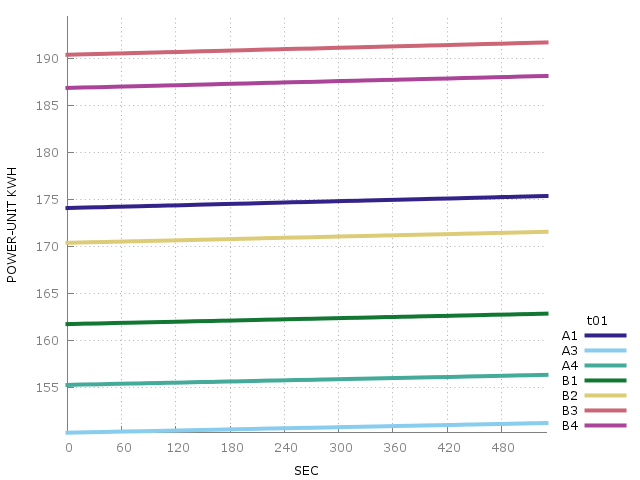
\includegraphics[width=3.1in]{gnu/ld/plot/PowerKWH_t01.png}}
   \fbox{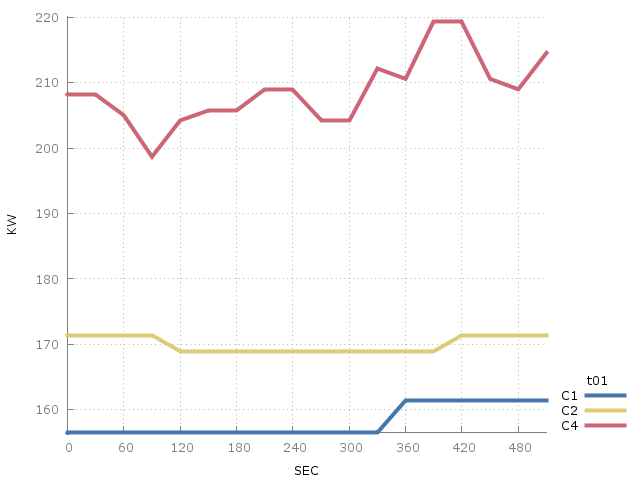
\includegraphics[width=3.1in]{gnu/ld/plot/KW_t01.png}}\\
   \centerline{\bfseries Trial 2---Low-Density Workload---Power-Unit kWh Increase \& Chiller KW}\\
   \fbox{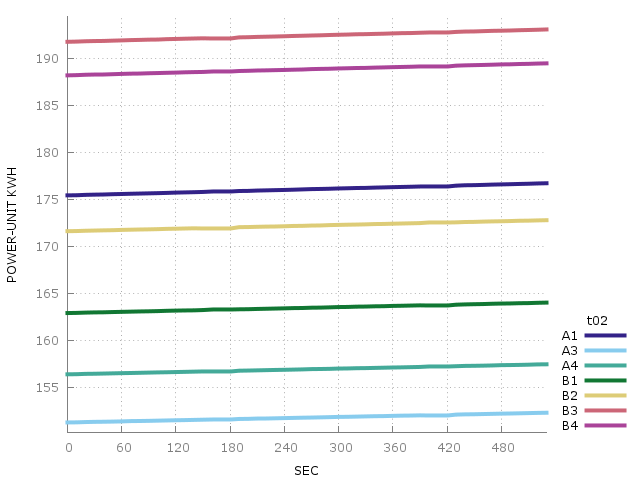
\includegraphics[width=3.1in]{gnu/ld/plot/PowerKWH_t02.png}}
   \fbox{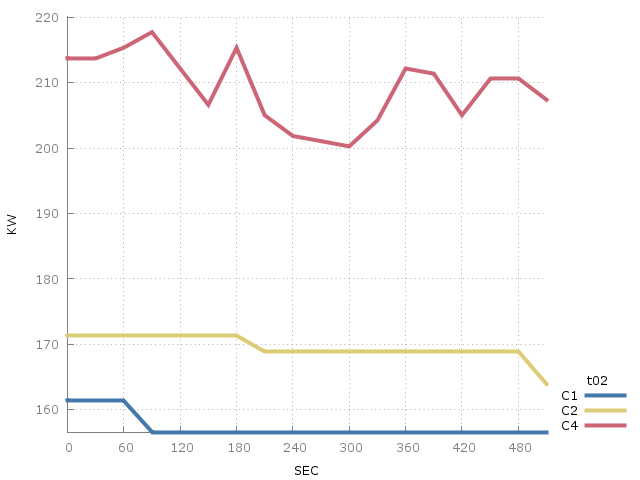
\includegraphics[width=3.1in]{gnu/ld/plot/KW_t02.png}}\\
   \centerline{\bfseries Trial 3---Low-Density Workload---Power-Unit kWh Increase \& Chiller KW}\\
   \fbox{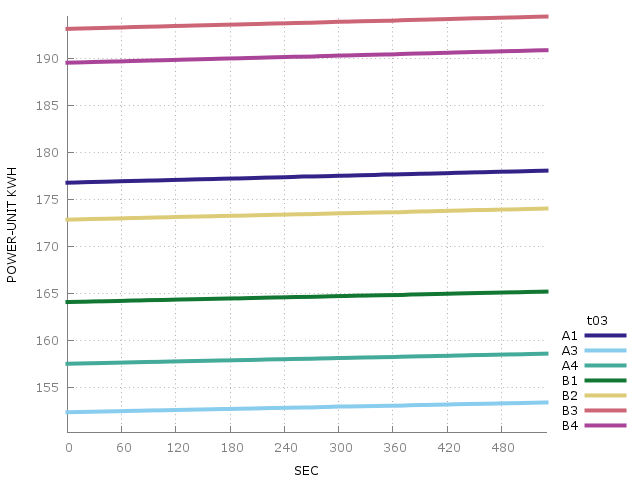
\includegraphics[width=3.1in]{gnu/ld/plot/PowerKWH_t03.png}}
   \fbox{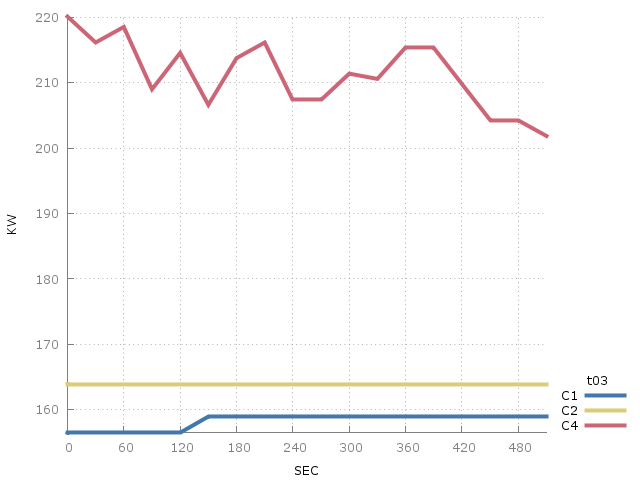
\includegraphics[width=3.1in]{gnu/ld/plot/KW_t03.png}}\\

 \end{tabular}

 \caption{The IT cooling load for the Chillers in use, specified in kilowatts (left), and the Power Unit kWh increase (right).}
\end{figure}
%%%%%%%%%%%%%%%%%%%%%%%%%%%%%%%%%%%%%%%%%%%%%%%%%%%%%%%%%%%%%%%%%%%%%%%%%%%%%%%


%%%%%%%%%%%%%%%%%%%%%%%%%%%%%%%%%%%%%%%%%%%%%%%%%%%%%%%%%%%%%%%%%%%%%%%%%%%%%%%
\begin{figure}[!h]

 \begin{tabular}{l}
   \centerline{\bfseries Trial 1---Low-Density Workload---TMU Utilization}\\
   \fbox{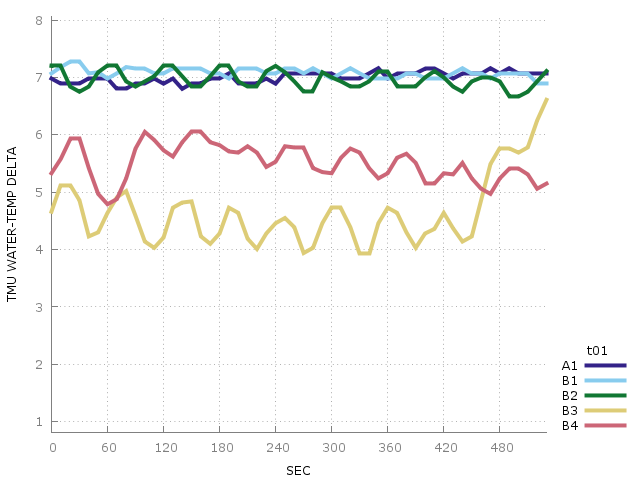
\includegraphics[width=3.1in]{gnu/ld/plot/TMU_WTD_t01.png}}
   \fbox{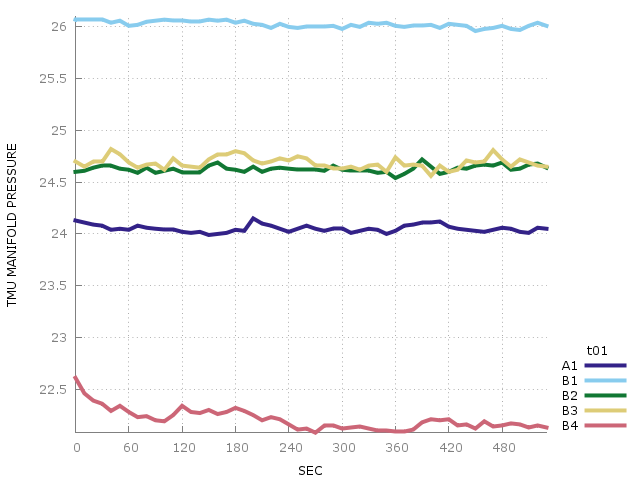
\includegraphics[width=3.1in]{gnu/ld/plot/ManifoldPress_t01.png}}\\
   \centerline{\bfseries Trial 2---Low-Density Workload---TMU Utilization}\\
   \fbox{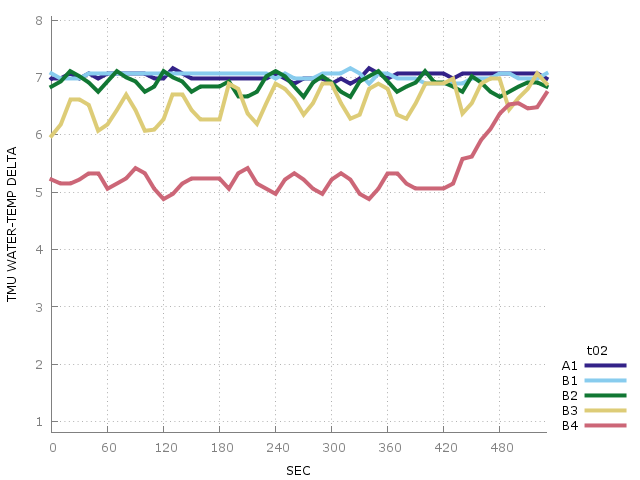
\includegraphics[width=3.1in]{gnu/ld/plot/TMU_WTD_t02.png}}
   \fbox{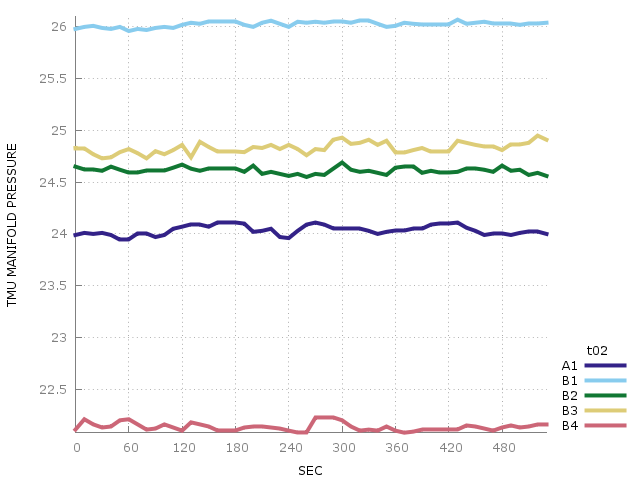
\includegraphics[width=3.1in]{gnu/ld/plot/ManifoldPress_t02.png}}\\
   \centerline{\bfseries Trial 3---Low-Density Workload---TMU Utilization}\\
   \fbox{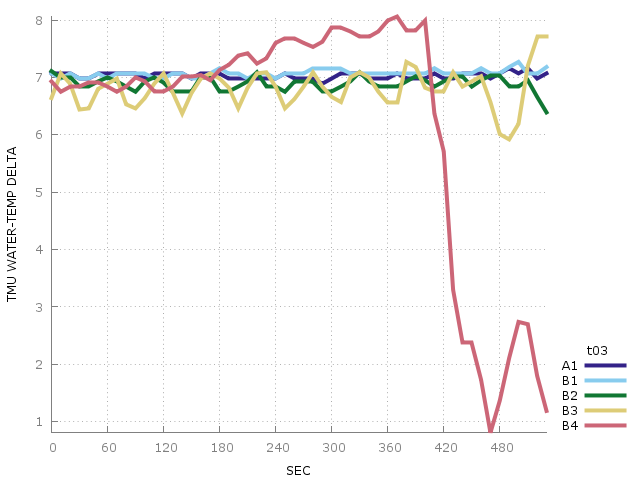
\includegraphics[width=3.1in]{gnu/ld/plot/TMU_WTD_t03.png}}
   \fbox{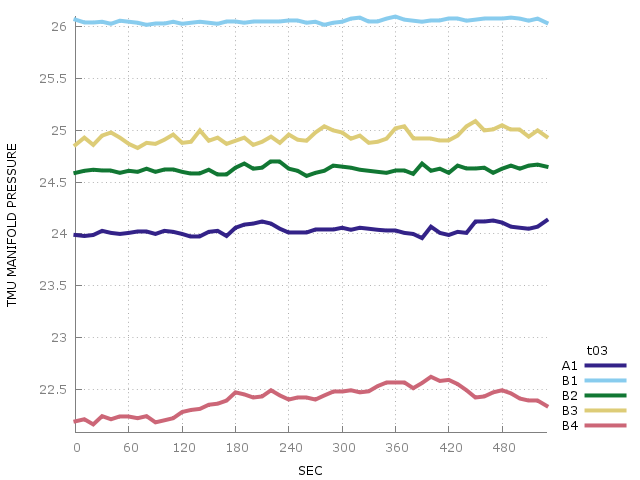
\includegraphics[width=3.1in]{gnu/ld/plot/ManifoldPress_t03.png}}\\

 \end{tabular}

 \caption{TMU utilization. The water temperature delta (WTD), which is obtained by subtracting inlet from outlet temperatures, and the pressure of the hot/cold liquid distribution manifold (right).}
\end{figure}
%%%%%%%%%%%%%%%%%%%%%%%%%%%%%%%%%%%%%%%%%%%%%%%%%%%%%%%%%%%%%%%%%%%%%%%%%%%%%%%

%%%%%%%%%%%%%%%%%%%%%%%%%%%%%%%%%%%%%%%%%%%%%%%%%%%%%%%%%%%%%%%%%%%%%%%%%%%%%%%
\begin{figure}[!h]

 \begin{tabular}{l}
   \centerline{\bfseries Trial 1---Low-Density Workload---Chiller Utilization}\\
   \fbox{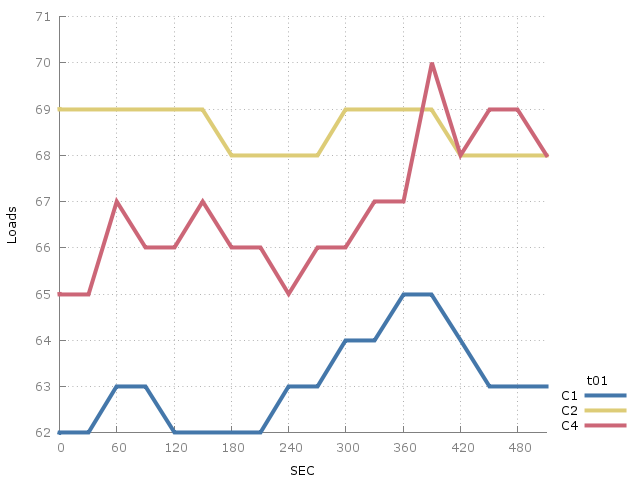
\includegraphics[width=3.1in]{gnu/ld/plot/Loads_t01.png}}
   \fbox{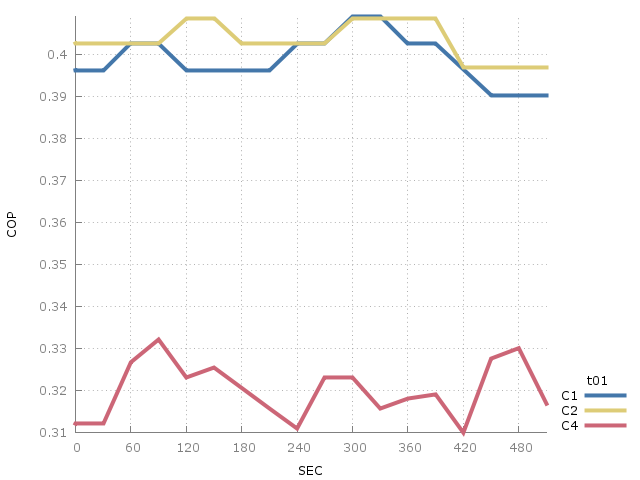
\includegraphics[width=3.1in]{gnu/ld/plot/COP_t01.png}}\\
   \centerline{\bfseries Trial 2---Low-Density Workload---Chiller Utilization}\\
   \fbox{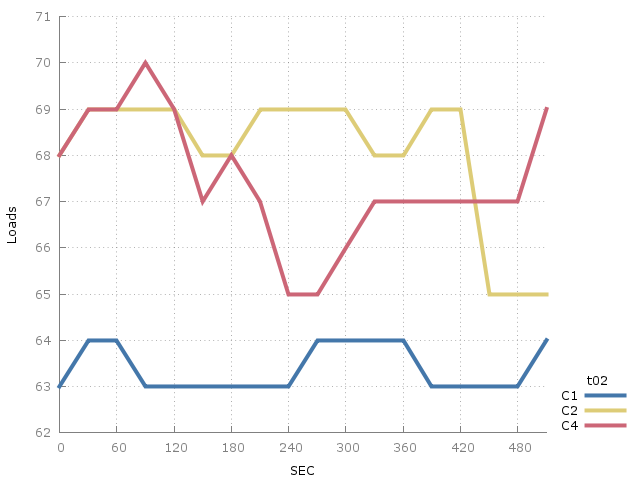
\includegraphics[width=3.1in]{gnu/ld/plot/Loads_t02.png}}
   \fbox{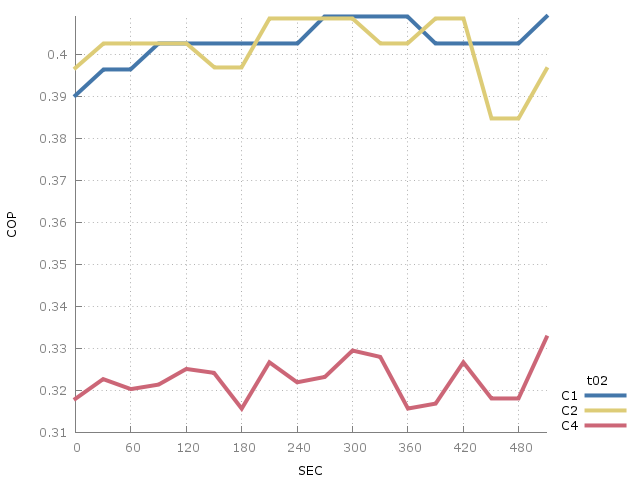
\includegraphics[width=3.1in]{gnu/ld/plot/COP_t02.png}}\\
   \centerline{\bfseries Trial 3---Low-Density Workload---Chiller Utilization}\\
   \fbox{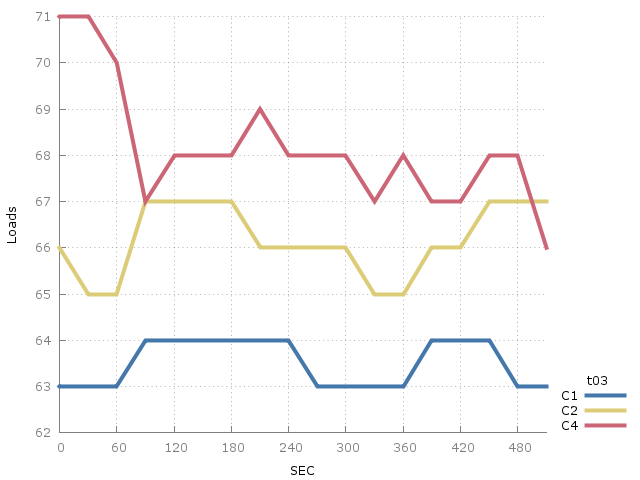
\includegraphics[width=3.1in]{gnu/ld/plot/Loads_t03.png}}
   \fbox{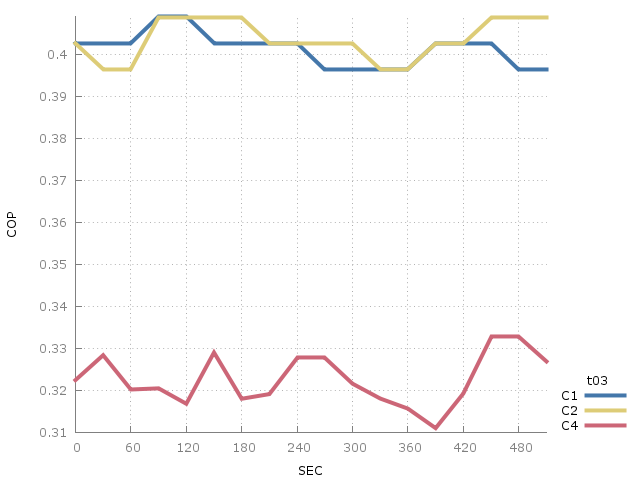
\includegraphics[width=3.1in]{gnu/ld/plot/COP_t03.png}}\\

 \end{tabular}

 \caption{Chiller Loads (left) and Chiller coefficient of performance (COP, right).} 
\end{figure} 
%%%%%%%%%%%%%%%%%%%%%%%%%%%%%%%%%%%%%%%%%%%%%%%%%%%%%%%%%%%%%%%%%%%%%%%%%%%%%%%

%%%%%%%%%%%%%%%%%%%%%%%%%%%%%%%%%%%%%%%%%%%%%%%%%%%%%%%%%%%%%%%%%%%%%%%%%%%%%%%
\begin{figure}[!h]

 \begin{tabular}{l}
   \centerline{\bfseries Trial 1---Low-Density Workload---Chiller Utilization}\\
   \fbox{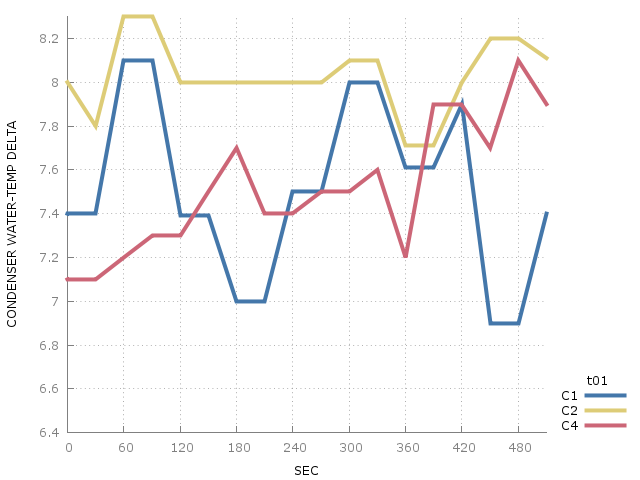
\includegraphics[width=3.1in]{gnu/ld/plot/C_WTD_t01.png}}
   \fbox{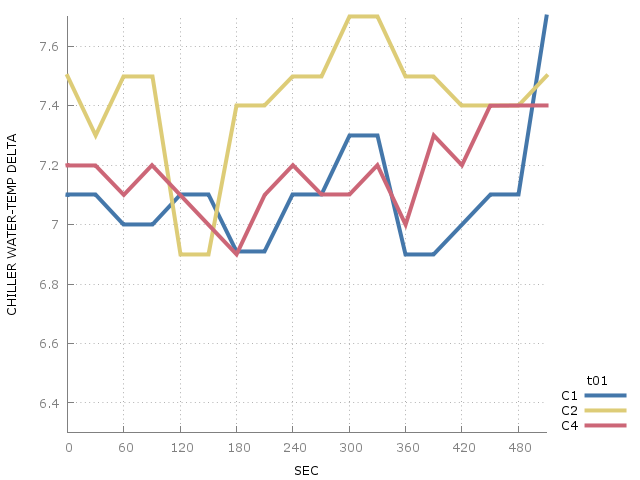
\includegraphics[width=3.1in]{gnu/ld/plot/CH_WTD_t01.png}}\\
   \centerline{\bfseries Trial 2---Low-Density Workload---Chiller Utilization}\\
   \fbox{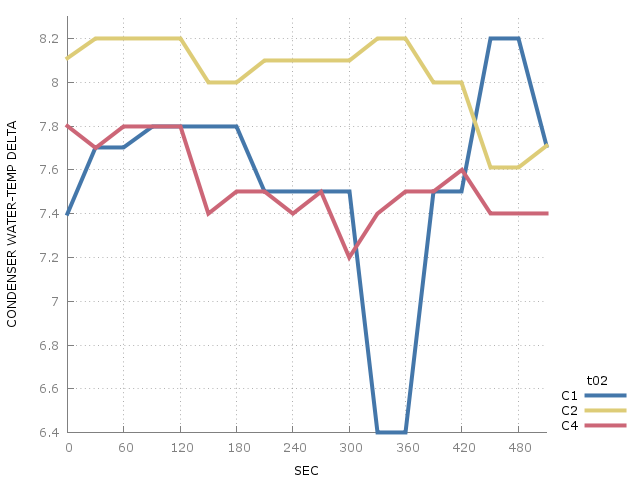
\includegraphics[width=3.1in]{gnu/ld/plot/C_WTD_t02.png}}
   \fbox{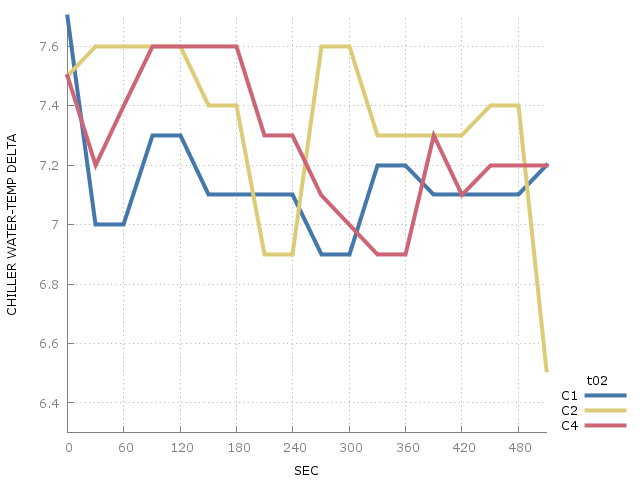
\includegraphics[width=3.1in]{gnu/ld/plot/CH_WTD_t02.png}}\\
   \centerline{\bfseries Trial 3---Low-Density Workload---Chiller Utilization}\\
   \fbox{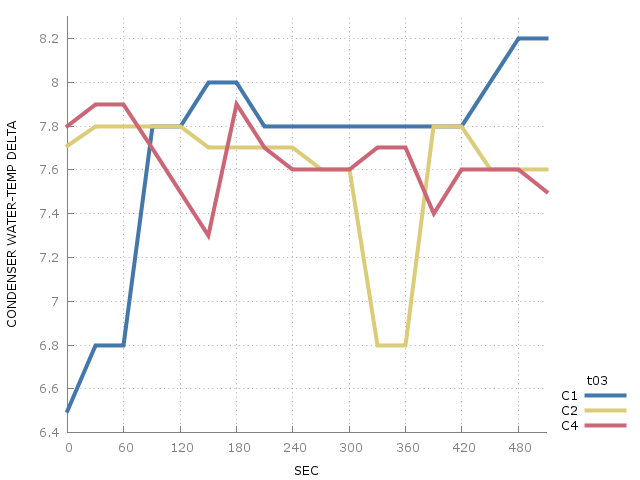
\includegraphics[width=3.1in]{gnu/ld/plot/C_WTD_t03.png}}
   \fbox{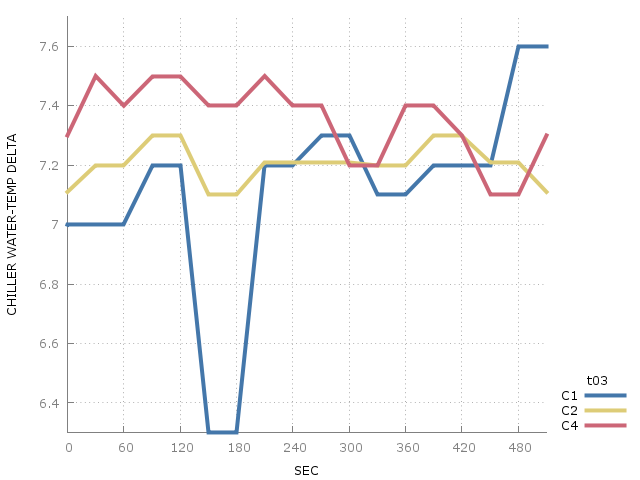
\includegraphics[width=3.1in]{gnu/ld/plot/CH_WTD_t03.png}}\\

 \end{tabular}

 \caption{Chiller utilization. The condenser water-temperature delta ($LCWT-ECWT$, left), and the Chiller water-temperature delta ($ECHWT-LCHWT$, right).}
\end{figure}

%%%%%%%%%%%%%%%%%%%%%%%%%%%%%%%%%%%%%%%%%%%%%%%%%%%%%%%%%%%%%%%%%%%%%%%%%%%%%%%
\begin{landscape}
%%%%%%%%%%%%%%%%%%%%%%%%%%%%%%%%%%%%%%%%%%%%%%%%%%%%%%%%%%%%%%%%%%%%%%%%%%%%%%%
%%%%%%%%%%%%%%%%%%%%%%%%%%%%%%%%%%%%%%%%%%%%%%%%%%%%%%%%%%%%%%%%%%%%%%%%%%%%%%%
\begin{figure}[!h]
  \centering
   \fbox{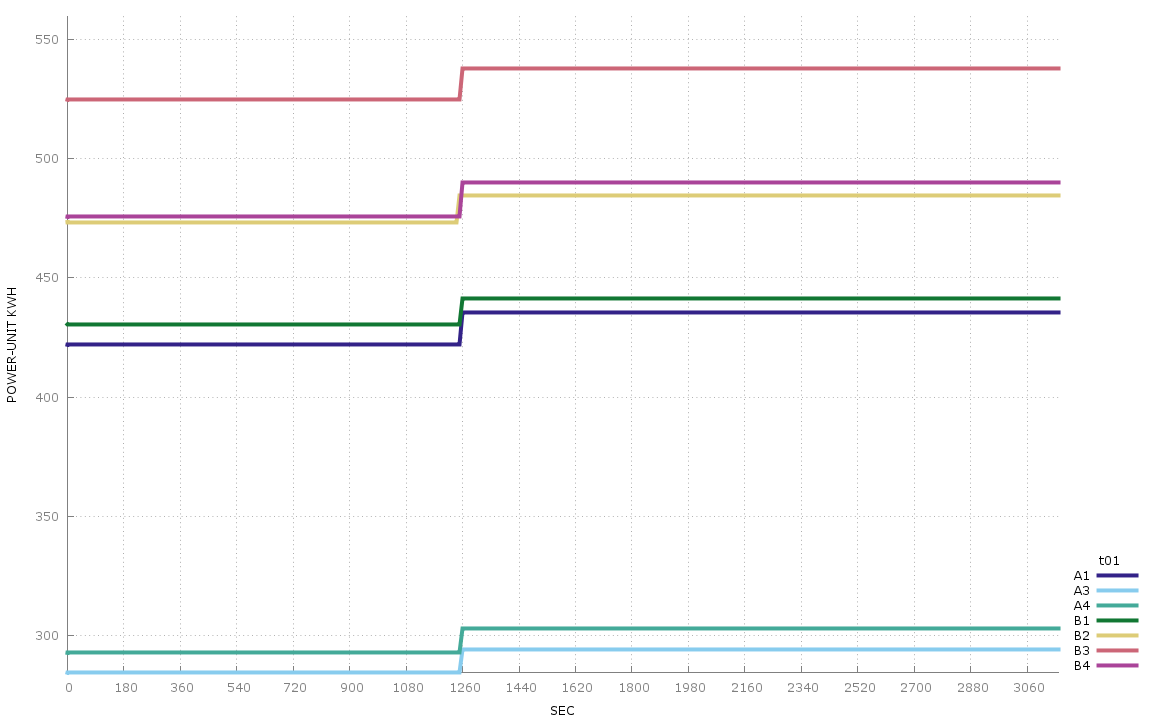
\includegraphics[width=9in]{gnu/hd/plot/PowerKWH_t01.png}}

    \caption{Trial 1---High-Density Workload---kWh Increase}
\end{figure}
%%%%%%%%%%%%%%%%%%%%%%%%%%%%%%%%%%%%%%%%%%%%%%%%%%%%%%%%%%%%%%%%%%%%%%%%%%%%%%%
\begin{figure}[!h]
  \centering
   \fbox{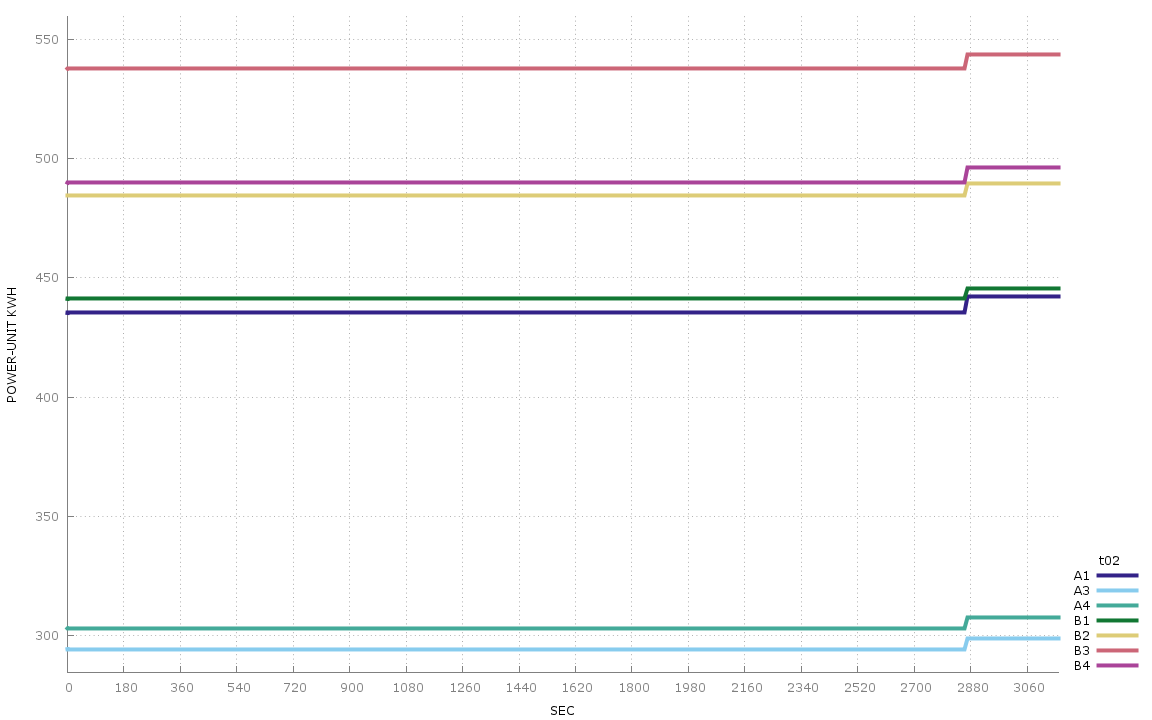
\includegraphics[width=9in]{gnu/hd/plot/PowerKWH_t02.png}}

    \caption{Trial 2---High-Density Workload---kWh Increase}
\end{figure}
%%%%%%%%%%%%%%%%%%%%%%%%%%%%%%%%%%%%%%%%%%%%%%%%%%%%%%%%%%%%%%%%%%%%%%%%%%%%%%%
\begin{figure}[!h]
  \centering
   \fbox{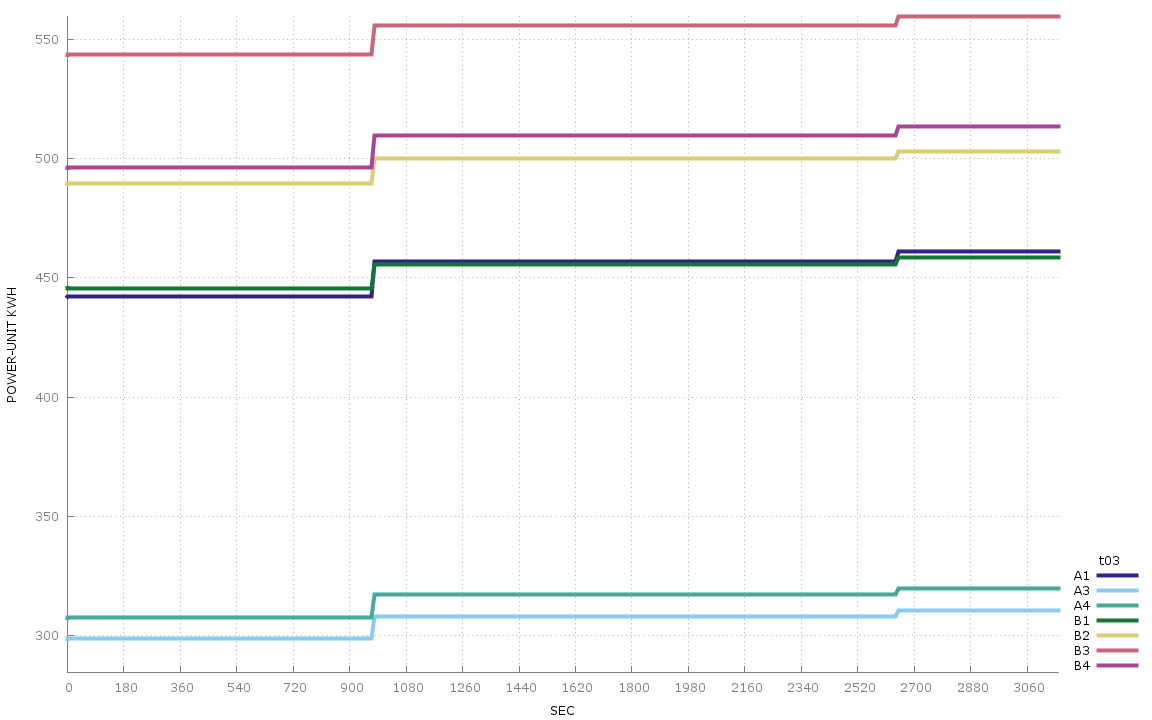
\includegraphics[width=9in]{gnu/hd/plot/PowerKWH_t03.png}}

    \caption{Trial 3---High-Density Workload---kWh Increase}
\end{figure}
%%%%%%%%%%%%%%%%%%%%%%%%%%%%%%%%%%%%%%%%%%%%%%%%%%%%%%%%%%%%%%%%%%%%%%%%%%%%%%%
\begin{figure}[!h]
  \centering
   \fbox{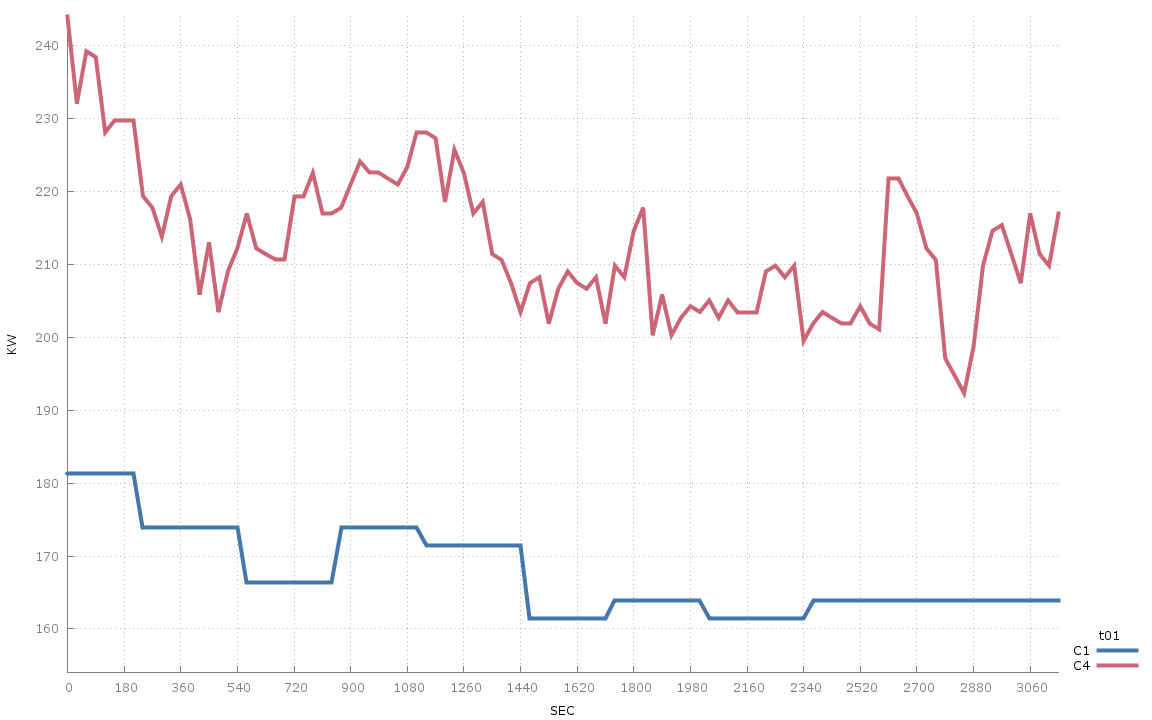
\includegraphics[width=9in]{gnu/hd/plot/KW_t01.png}}

    \caption{Trial 1---High-Density Workload---Chiller KW}
\end{figure}
%%%%%%%%%%%%%%%%%%%%%%%%%%%%%%%%%%%%%%%%%%%%%%%%%%%%%%%%%%%%%%%%%%%%%%%%%%%%%%%
\begin{figure}[!h]
  \centering
   \fbox{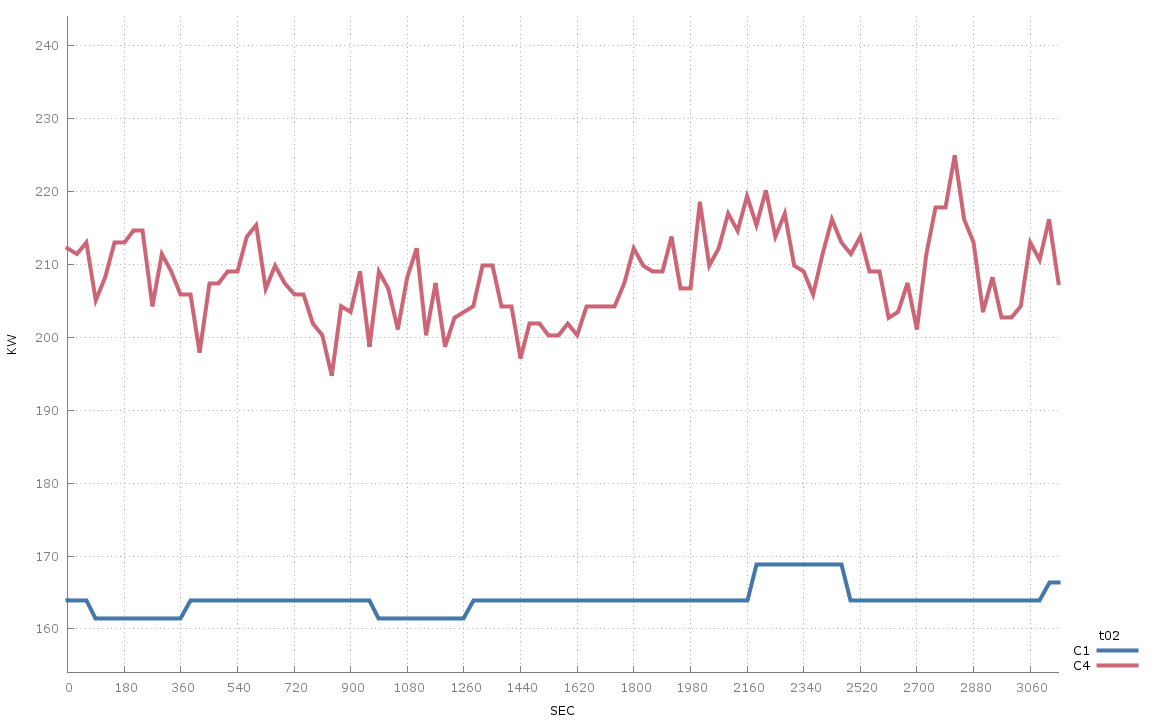
\includegraphics[width=9in]{gnu/hd/plot/KW_t02.png}}
%%%%%%%%%%%%%%%%%%%%%%%%%%%%%%%%%%%%%%%%%%%%%%%%%%%%%%%%%%%%%%%%%%%%%%%%%%%%%%%
    \caption{Trial 2---High-Density Workload---Chiller KW}
\end{figure}
\begin{figure}[!h]
  \centering
   \fbox{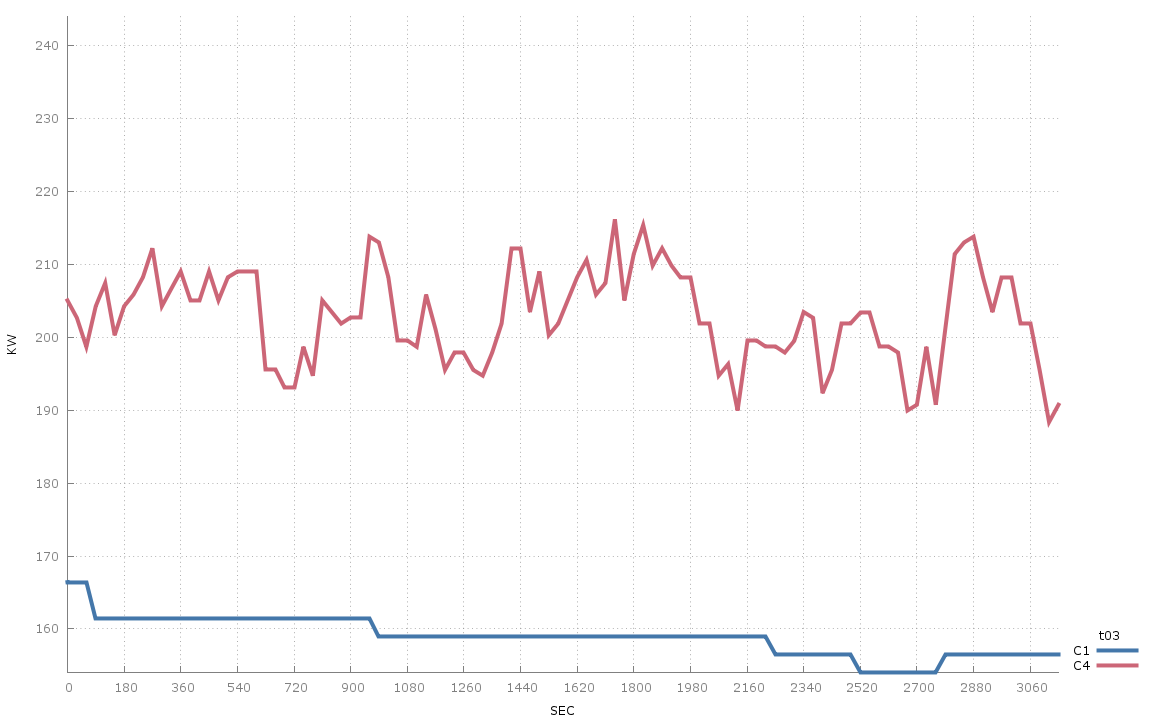
\includegraphics[width=9in]{gnu/hd/plot/KW_t03.png}}

    \caption{Trial 3---High-Density Workload---Chiller KW}
\end{figure}
%%%%%%%%%%%%%%%%%%%%%%%%%%%%%%%%%%%%%%%%%%%%%%%%%%%%%%%%%%%%%%%%%%%%%%%%%%%%%%%
\begin{figure}[!h]
  \centering
   \fbox{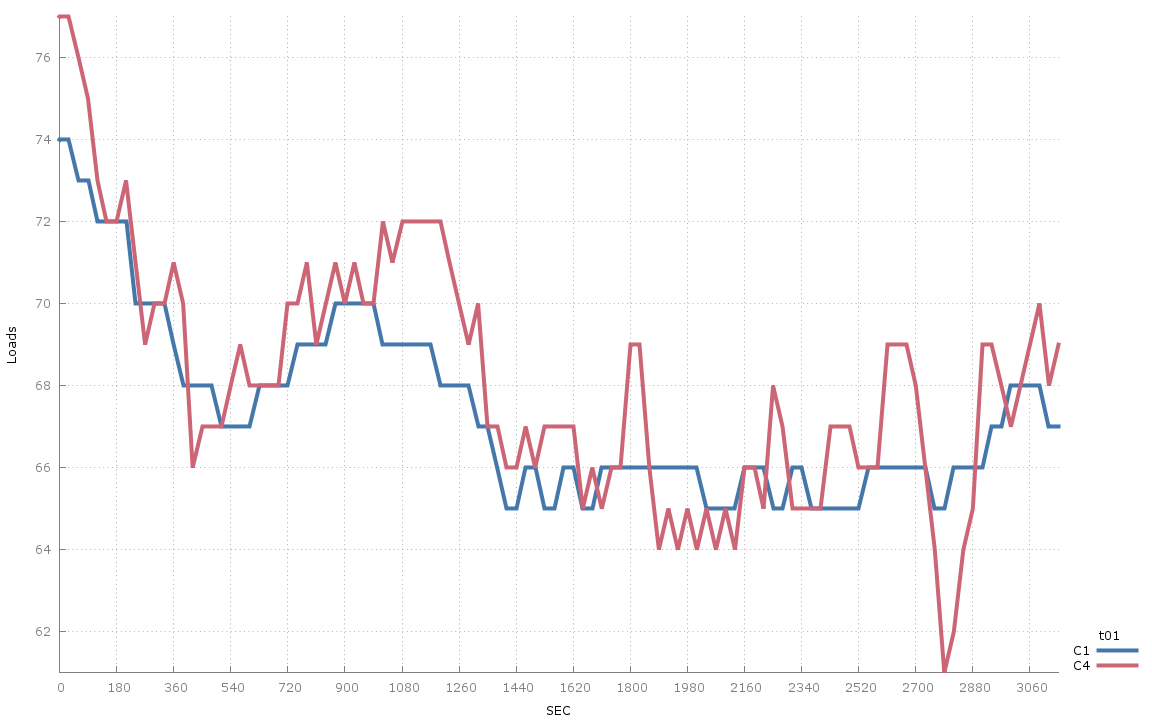
\includegraphics[width=9in]{gnu/hd/plot/Loads_t01.png}}

    \caption{Trial 1---High-Density Workload---Chiller Loads}
\end{figure}
%%%%%%%%%%%%%%%%%%%%%%%%%%%%%%%%%%%%%%%%%%%%%%%%%%%%%%%%%%%%%%%%%%%%%%%%%%%%%%%
\begin{figure}[!h]
  \centering
   \fbox{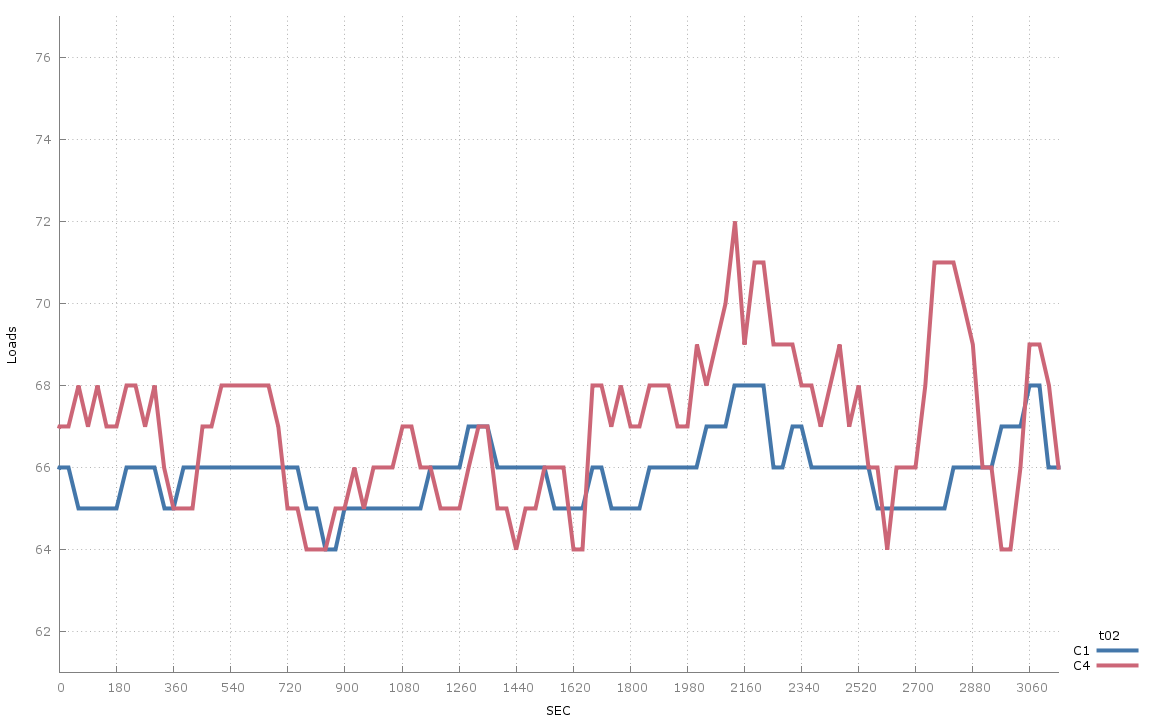
\includegraphics[width=9in]{gnu/hd/plot/Loads_t02.png}}

    \caption{Trial 2---High-Density Workload---Chiller Loads}
\end{figure}
%%%%%%%%%%%%%%%%%%%%%%%%%%%%%%%%%%%%%%%%%%%%%%%%%%%%%%%%%%%%%%%%%%%%%%%%%%%%%%%
\begin{figure}[!h]
  \centering
   \fbox{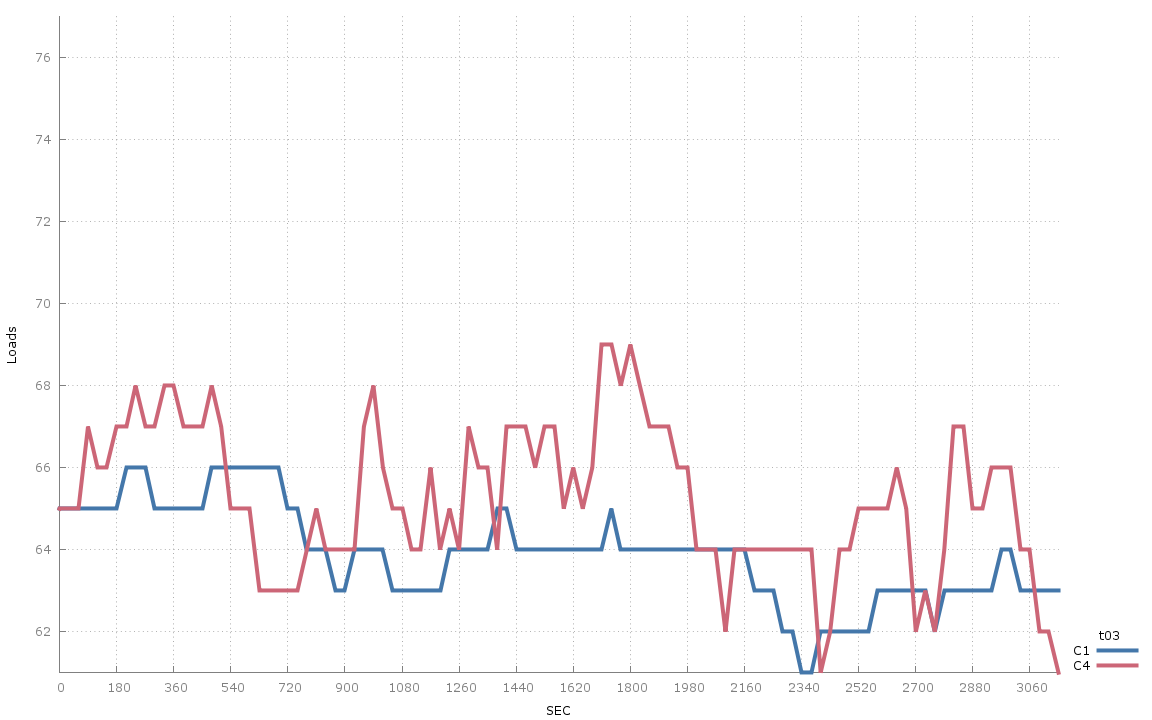
\includegraphics[width=9in]{gnu/hd/plot/Loads_t03.png}}

    \caption{Trial 3---High-Density Workload---Chiller Loads}
\end{figure}
%%%%%%%%%%%%%%%%%%%%%%%%%%%%%%%%%%%%%%%%%%%%%%%%%%%%%%%%%%%%%%%%%%%%%%%%%%%%%%%
\begin{figure}[!h]
  \centering
   \fbox{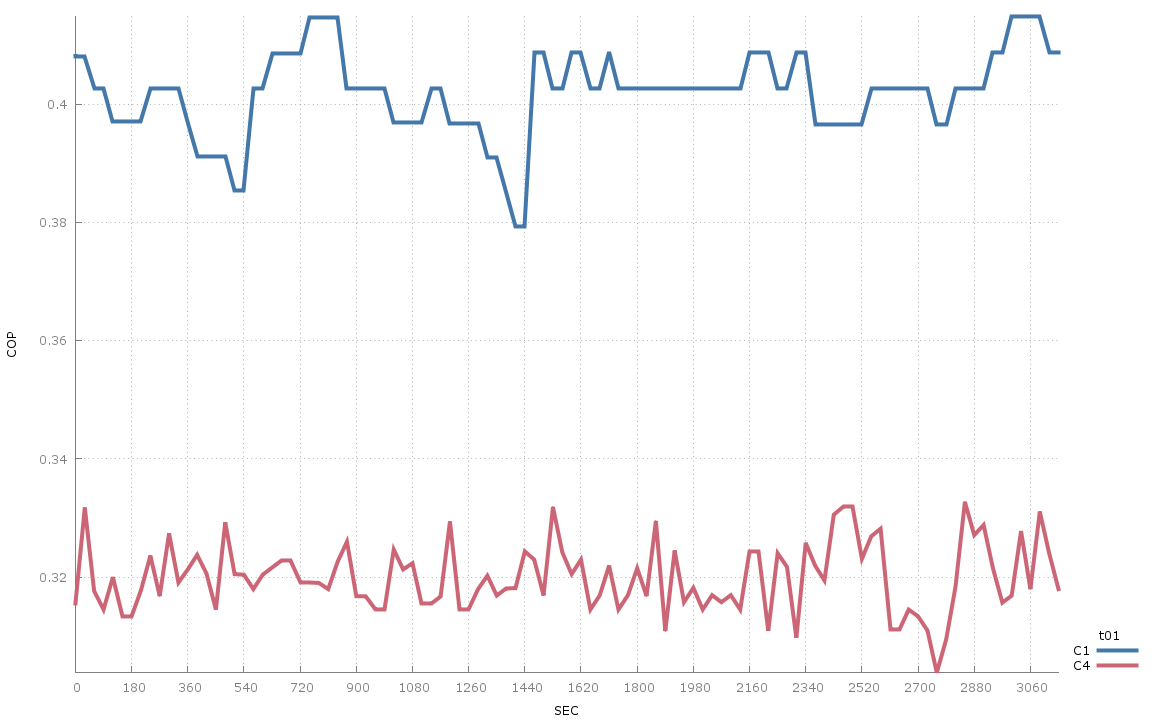
\includegraphics[width=9in]{gnu/hd/plot/COP_t01.png}}

    \caption{Trial 1---High-Density Workload---Chiller COP}
\end{figure}
%%%%%%%%%%%%%%%%%%%%%%%%%%%%%%%%%%%%%%%%%%%%%%%%%%%%%%%%%%%%%%%%%%%%%%%%%%%%%%%
\begin{figure}[!h]
  \centering
   \fbox{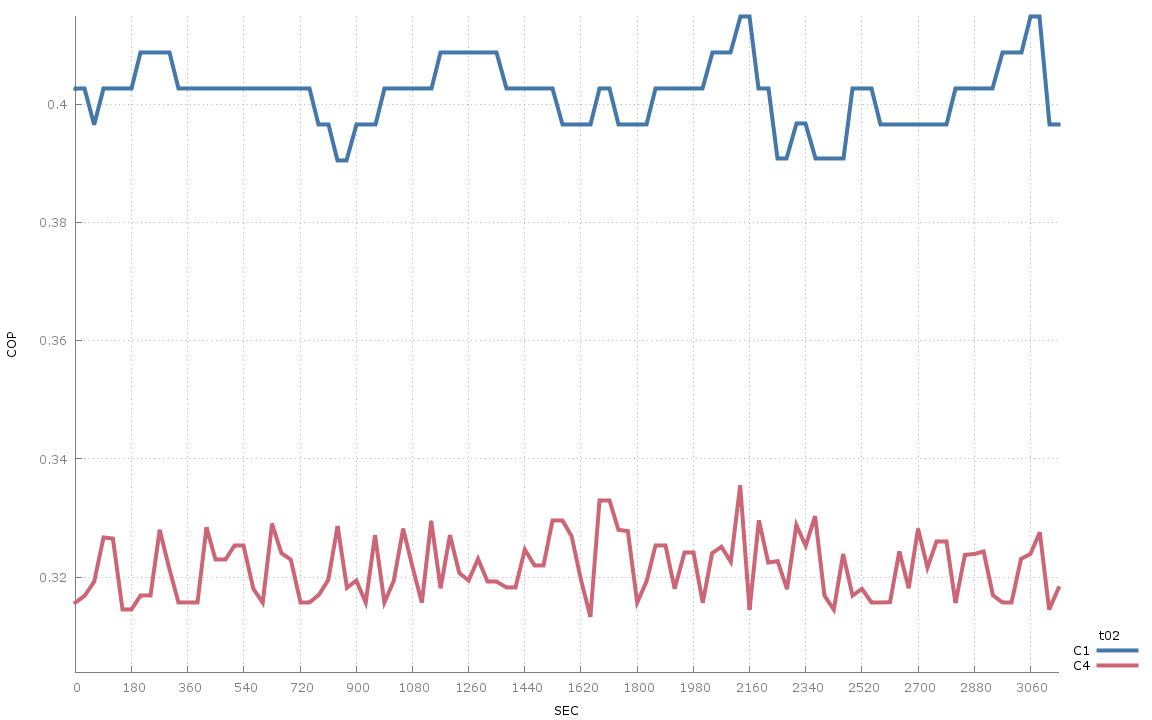
\includegraphics[width=9in]{gnu/hd/plot/COP_t02.png}}

    \caption{Trial 2---High-Density Workload---Chiller COP}
\end{figure}
%%%%%%%%%%%%%%%%%%%%%%%%%%%%%%%%%%%%%%%%%%%%%%%%%%%%%%%%%%%%%%%%%%%%%%%%%%%%%%%
\begin{figure}[!h]
  \centering
   \fbox{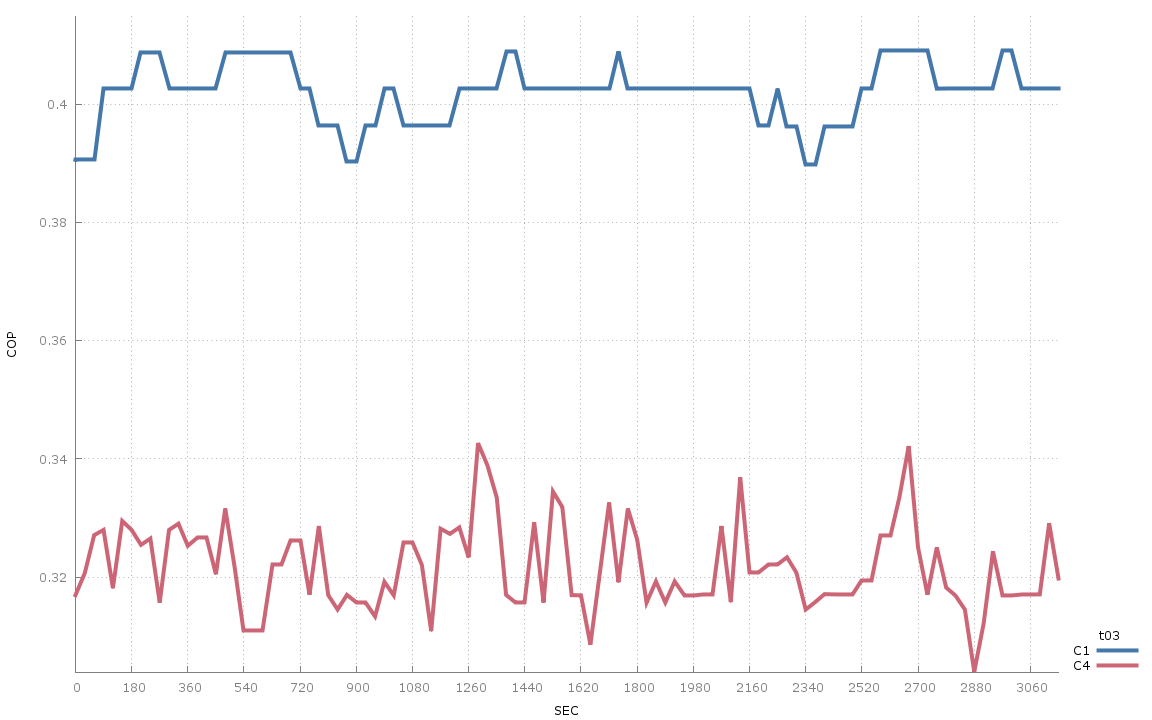
\includegraphics[width=9in]{gnu/hd/plot/COP_t03.png}}

    \caption{Trial 3---High-Density Workload---Chiller COP}
\end{figure}
%%%%%%%%%%%%%%%%%%%%%%%%%%%%%%%%%%%%%%%%%%%%%%%%%%%%%%%%%%%%%%%%%%%%%%%%%%%%%%%
\begin{figure}[!h]
  \centering
   \fbox{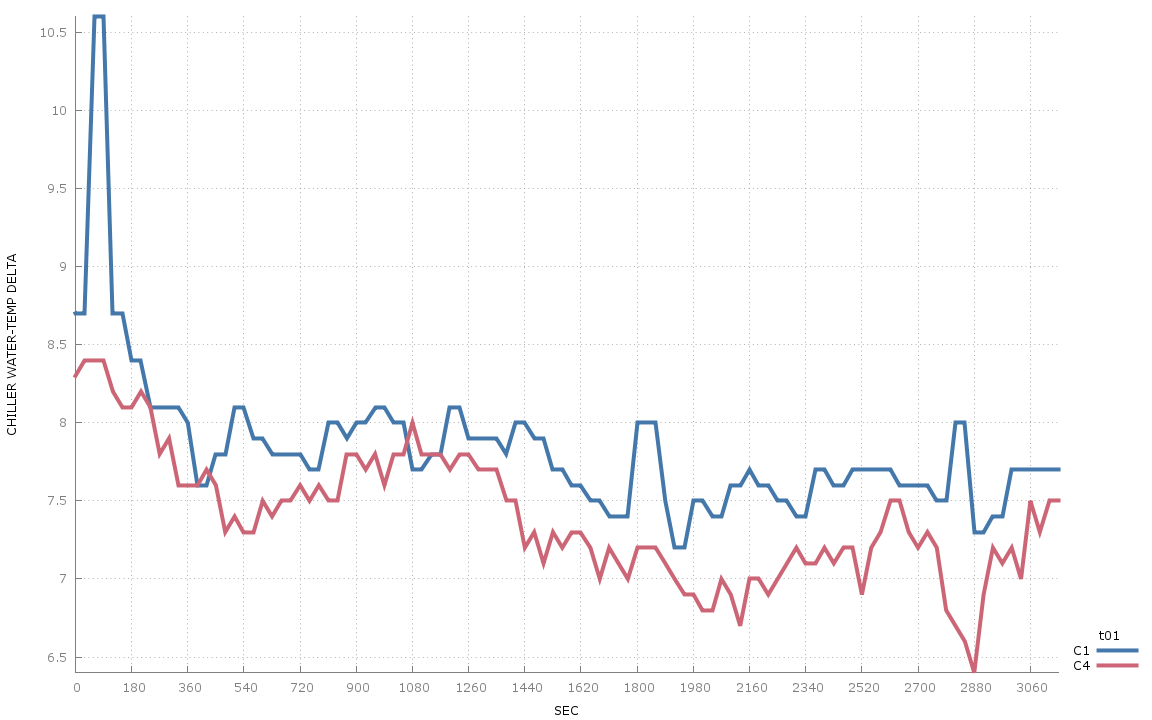
\includegraphics[width=9in]{gnu/hd/plot/CH_WTD_t01.png}}

    \caption{Trial 1---High-Density Workload---Chiller Water Temperature Delta}
\end{figure}
%%%%%%%%%%%%%%%%%%%%%%%%%%%%%%%%%%%%%%%%%%%%%%%%%%%%%%%%%%%%%%%%%%%%%%%%%%%%%%%
\begin{figure}[!h]
  \centering
   \fbox{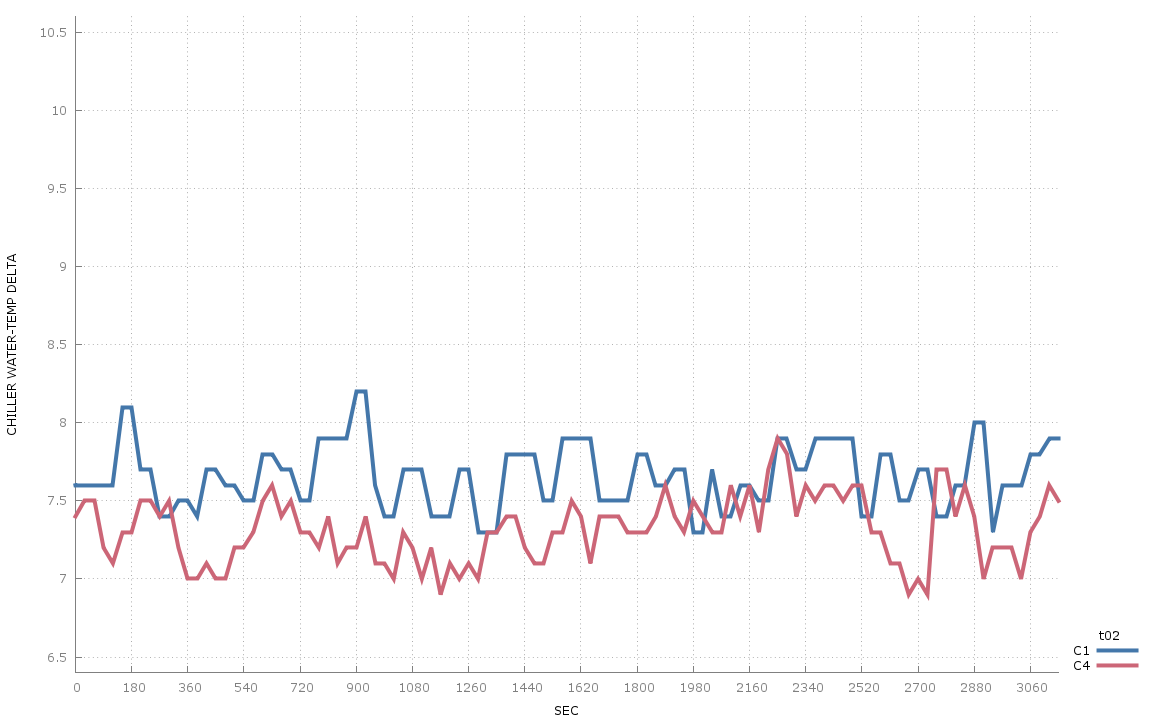
\includegraphics[width=9in]{gnu/hd/plot/CH_WTD_t02.png}}

    \caption{Trial 2---High-Density Workload---Chiller Water Temperature Delta}
\end{figure}
%%%%%%%%%%%%%%%%%%%%%%%%%%%%%%%%%%%%%%%%%%%%%%%%%%%%%%%%%%%%%%%%%%%%%%%%%%%%%%%
\begin{figure}[!h]
  \centering
   \fbox{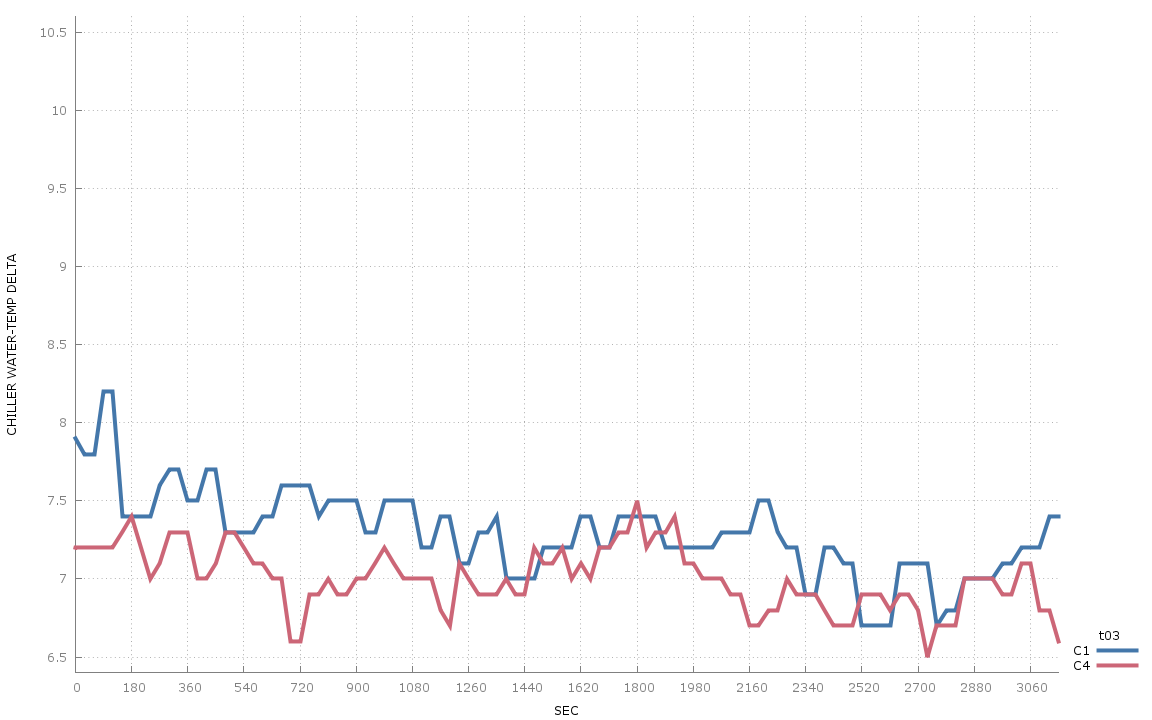
\includegraphics[width=9in]{gnu/hd/plot/CH_WTD_t03.png}}

    \caption{Trial 3---High-Density Workload---Chiller Water Temperature Delta}
\end{figure}
%%%%%%%%%%%%%%%%%%%%%%%%%%%%%%%%%%%%%%%%%%%%%%%%%%%%%%%%%%%%%%%%%%%%%%%%%%%%%%%

%%%%%%%%%%%%%%%%%%%%%%%%%%%%%%%%%%%%%%%%%%%%%%%%%%%%%%%%%%%%%%%%%%%%%%%%%%%%%%%
\end{landscape}
%%%%%%%%%%%%%%%%%%%%%%%%%%%%%%%%%%%%%%%%%%%%%%%%%%%%%%%%%%%%%%%%%%%%%%%%%%%%%%%


\clearpage
%\nocite{*}
\bibliographystyle{plain}
\bibliography{report}

%%%%%%%%%%%%%%%%%%%%%%%%%%%%%%%%%%%%%%%%%%%%%%%%%%%%%%%%%%%%%%%%%%%%%%%%%%%%%%%
%%%%%%%%%%%%%%%%%%%%%%%%%%%%%%%%%%%%%%%%%%%%%%%%%%%%%%%%%%%%%%%%%%%%%%%%%%%%%%%
%%%%%%%%%%%%%%%%%%%%%%%%%%%%%%%%%%%%%%%%%%%%%%%%%%%%%%%%%%%%%%%%%%%%%%%%%%%%%%%
\end{document}
%%%%%%%%%%%%%%%%%%%%%%%%%%%%%%%%%%%%%%%%%%%%%%%%%%%%%%%%%%%%%%%%%%%%%%%%%%%%%%%
%%%%%%%%%%%%%%%%%%%%%%%%%%%%%%%%%%%%%%%%%%%%%%%%%%%%%%%%%%%%%%%%%%%%%%%%%%%%%%%
%%%%%%%%%%%%%%%%%%%%%%%%%%%%%%%%%%%%%%%%%%%%%%%%%%%%%%%%%%%%%%%%%%%%%%%%%%%%%%%
  \item Give a complete performance diagnosis; gathering total energy consumption and rack cooling effort into \emph{intensity} metrics, as in \cite{Karavanic2011}.
   \item Compare how the two air-cooled racks ($A_3,A_4$) faired with the LD workload against the water-cooled racks ($A_1,B_1,\dots B_4$).
   \item Showcase PerfTrack, as in \cite{Karavanic2010}.



   \vspace{0.5cm}
   \centerline{Average, per node, air inlet temperatures (left table, below) and air exchange temperatures (right table, below).}
   \vspace{0.5cm}
\input{src/table/ld/nodeair_intemp7.tex}\hfill
\input{src/table/ld/nodeair_exchangetemp7.tex}
    \caption{Low-Density Workload Energy}
\end{figure}
%%%%%%%%%%%%%%%%%%%%%%%%%%%%%%%%%%%%%%%%%%%%%%%%%%%%%%%%%%%%%%%%%%%%%%%%%%%%%%%
\end{landscape}
%%%%%%%%%%%%%%%%%%%%%%%%%%%%%%%%%%%%%%%%%%%%%%%%%%%%%%%%%%%%%%%%%%%%%%%%%%%%%%%

%%%%%%%%%%%%%%%%%%%%%%%%%%%%%%%%%%%%%%%%%%%%%%%%%%%%%%%%%%%%%%%%%%%%%%%%%%%%%%%

%%%%%%%%%%%%%%%%%%%%%%%%%%%%%%%%%%%%%%%%%%%%%%%%%%%%%%%%%%%%%%%%%%%%%%%%%%%%%%%
\begin{table}[!h]
  \centering
   \centerline{\bfseries High-Density Workload}\\\hline
   \vspace{1cm}
   \input{src/table/hd/powerunit_powerkwh7.tex}\\
   \vspace{0.5cm}
   \centerline{Total kWh increase.}
   \vspace{1cm}
   \input{src/table/hd/cpu_tempAvg.tex}\\
   \vspace{0.5cm}
   \centerline{Average Per-Node CPU Tempurature Average for Each Rack}
   \vspace{1cm}
   \input{src/table/hd/cpu_tempMax.tex}\\
   \vspace{0.5cm}
   \centerline{Average Per-Node CPU Tempurature Average for Each Rack}
   \vspace{1cm}
   \input{src/table/hd/nodeair_airdeltaAvg.tex}\\
   \vspace{0.5cm}
   \centerline{Average Per-Node Air Temperature Delta for Each Rack}
    \caption{High-Density Workload Energy}
\end{table}
%%%%%%%%%%%%%%%%%%%%%%%%%%%%%%%%%%%%%%%%%%%%%%%%%%%%%%%%%%%%%%%%%%%%%%%%%%%%%%%

\begin{figure}[!h]
  \centering
 \begin{tabular}{l}
   \centerline{\bfseries Low-Density Workload : kWh Increase}\\
   \flushleft
   \fbox{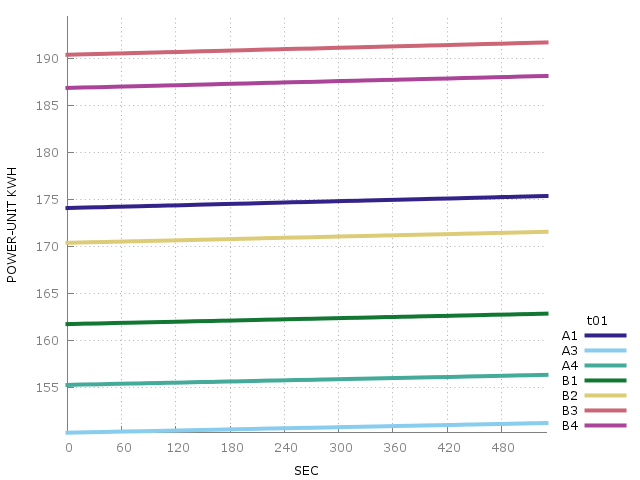
\includegraphics[width=3in]{gnu/ld/plot/PowerKWH_t01.png}}
   \fbox{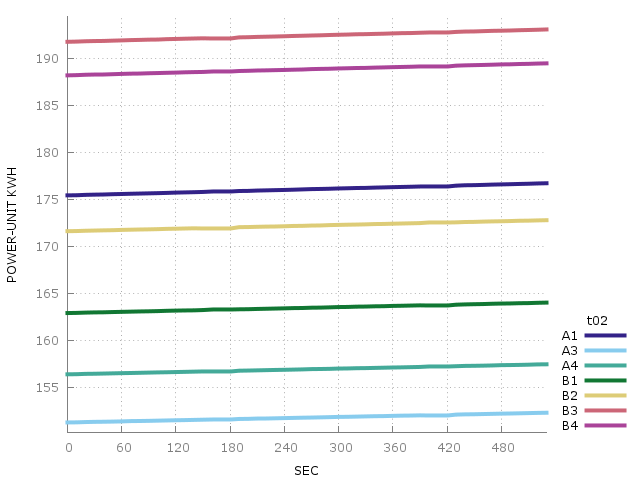
\includegraphics[width=3in]{gnu/ld/plot/PowerKWH_t02.png}}
   \fbox{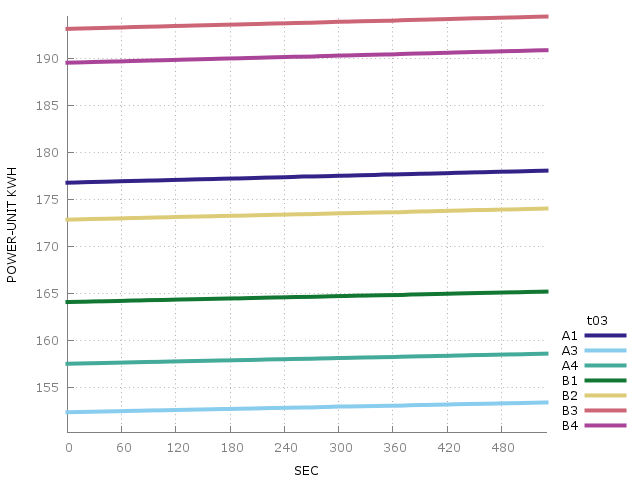
\includegraphics[width=3in]{gnu/ld/plot/PowerKWH_t03.png}}
    \end{tabular}

    \vspace{0.5cm}
   \begin{tabular}{r|ccccccc}\cline{2-8}
\tt PowerUnit PowerKWH&$\bf A1$&$\bf A3$&$\bf A4$&$\bf B1$&$\bf B2$&$\bf B3$&$\bf B4$\\\hline
\bf t01& 1.28& 1.03& 1.07& 1.11& 1.17& 1.31& 1.27\\
\bf t02& 1.28& 1.03& 1.06& 1.11& 1.17& 1.31& 1.27\\
\bf t03& 1.30& 1.05& 1.09& 1.13& 1.19& 1.33& 1.35\\
\hline
\tt Total PowerUnit& 1& 1& 1& 1& 1& 1& 1\\
\end{tabular}
\\
   \vspace{0.5cm}
   \begin{tabular}{r|ccccccc}\cline{2-8}
\tt CPU Temp&$\bf A1$&$\bf A3$&$\bf A4$&$\bf B1$&$\bf B2$&$\bf B3$&$\bf B4$\\\hline
\bf t01& 97.18& 83.52& 81.71& 100.15& 89.51& 94.54& 110.43\\
\bf t02& 104.83& 83.99& 82.30& 100.44& 89.75& 94.22& 111.05\\
\bf t03& 116.73& 83.89& 82.26& 100.42& 89.68& 97.33& 111.66\\
\hline
\tt Total CPU& 37& 41& 4& 5& 6& 4& 5\\
\end{tabular}
\\
\vspace{0.5cm}
   \begin{tabular}{r|ccccccc}\cline{2-8}
\tt NodeAir Delta&$\bf A1$&$\bf A3$&$\bf A4$&$\bf B1$&$\bf B2$&$\bf B3$&$\bf B4$\\\hline
\bf t01& 26.80& 26.20& 26.62& 24.52& 25.28& 24.37& 26.24\\
\bf t02& 27.43& 26.06& 26.44& 24.76& 25.28& 24.43& 26.92\\
\bf t03& 29.16& 25.87& 26.66& 24.16& 25.30& 24.38& 27.17\\
\hline
\tt Total NodeAir& 23& 23& 21& 25& 23& 23& 15\\
\end{tabular}
\\

   \caption{The sensor readings for CPU tempuratures had to be thresholded between 72 and 150 degrees F; many readings were negative, and some were ridiculously high. (Note: some nodes have more than one CPU.) Faulty sensor readings had to be filtered from the Node-Air Delta as well.}
\end{figure}


